%!TEX root = ../thesis.tex

\section{背景}
  近年,機械学習を活用した自律移動に関する研究が盛んに行われている.本研究室でも,機械学習を用いて画像に基づく人追従行動の生成に関する研究を行ってきた.

  パシンら\cite{pasin1}\cite{pasin2}\cite{pasin3}は,引き紐を利用して画像に基づく人追従行動を生成する手法を提案している.この手法では,深層強化学習\cite{hado}を活用しており,引き紐に取り付けられたポテンショメータでリンクの角度を取得し,それに応じた報酬をエージェント(ロボット)に与えて強化学習\cite{leslie}することで,画像に基づいて人追従する行動を生成できることを示した.
  \figref{Fig:pasin_system}にシステムの概要を示す.入力は画像で,出力は直進,左旋回,右旋回のいずれかの行動である.報酬は,引き紐を取り付けたリンクの角度に基づいており,人がロボットの正面に立つと報酬が高くなるように設定されている.ロボットは報酬が高くなるように行動を選択するため,引き紐を持つ人がロボットの正面にいない場合は,引き紐を持つ人がロボットの正面になるように,左旋回や右旋回といった行動を選択する.引き紐を持つ人が正面にいる場合は,ロボットは直進を選択する.さまざまな行動と画像に対して,リンクの角度に応じた報酬を与えることで,徐々に人を追従する適切な行動を選択していった.
  しかし,強化学習の特性により,行動の選択がランダムに探索される場合がある.その結果,報酬の低い行動が選択され,追従対象者が望まない行動が発生する可能性があった.また,カメラ画像に基づく人追従行動を獲得するまでに約20分かかり,その間にロボットは望まない行動を繰り返すため,追従対象者に比較的負担がかかるという問題があった.

\newpage

  \begin{figure}[h]
    \centering
    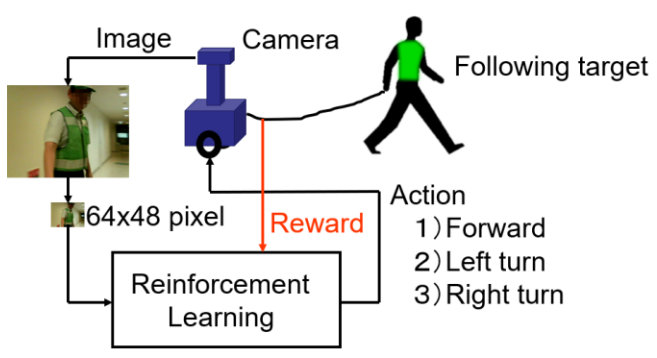
\includegraphics[keepaspectratio, scale=0.45] {images/pasin_system.png}
    \caption{Proposed method \cite{pasin1}}
    \label{Fig:pasin_system}
  \end{figure}

  岡田ら\cite{okada}は,強化学習のような教師なし学習ではなく,深層学習\cite{yann2}という教師あり学習を用いて画像に基づく人追従行動を生成する手法を提案している.この手法は,後述するBojarskiら\cite{bojarski}の技術(end-to-end学習)を人追従問題に応用しており,強化学習を使用していないため,ロボットの行動がランダムに選択されることはない.また,学習時はルールベース制御器でロボットを制御しているので,常に人を追従する.つまり,学習時にも人追従行動を獲得でき,強化学習を採用する手法と比べて追従対象者の負担が少ないというメリットがある.
  \figref{Fig:okada_system}にシステムの概要を示す.まず,学習時には,追従対象者が引き紐を操作する.引き紐にはパシンらと同様にポテンショメータが取り付けられており,ヨ―関節の変位角が0度となるようにロボットは直進や左旋回,右旋回のいずれかの行動で制御される.並行して,これらの行動とカメラ画像を深層学習器にオンラインでend-to-end学習する.学習後は,追従対象者が引き紐を操作しなくても,深層学習器によりカメラ画像を入力するだけで,出力は直進や左旋回,右旋回といった行動を選択する.つまり,学習時のルールベース制御器(引き紐による人追従行動)を模倣するような深層学習器(カメラ画像による人追従行動)になっている.

  これまで本研究室では,引き紐に依存した人追従行動を生成してきたが,2DLiDARの反射強度を利用することで同様の人追従行動を生成できる可能性がある.もし本研究の提案手法が有効であることが確認されれば,学習時のルールベース制御器に新たな選択肢が加わり,そのメリットが生まれる.

\newpage

  \begin{figure}[h]
    \centering
    \begin{minipage}[c]{100mm} 
        \centering
        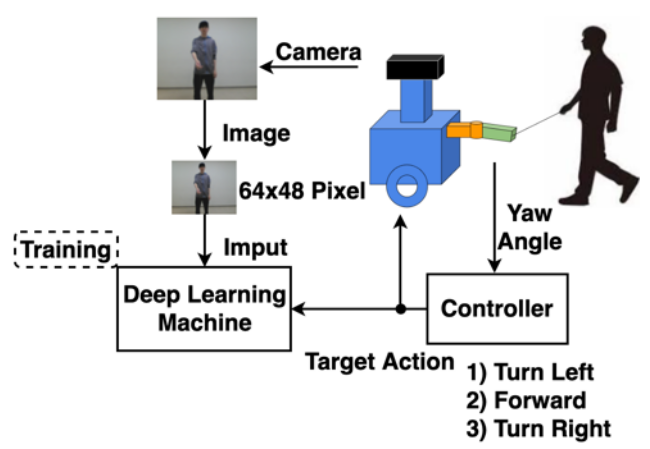
\includegraphics[width=100mm]{images/okada_learning_phase_system.png}
        \subcaption{Learning phase}
    \end{minipage} \\
    \vspace{1em} % 画像とキャプションの間にスペースを追加
    \begin{minipage}[c]{100mm} 
        \centering
        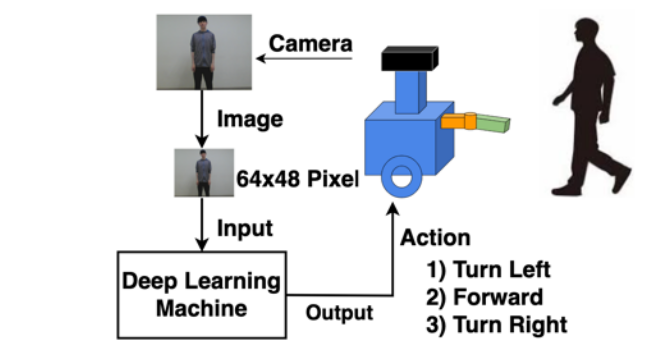
\includegraphics[width=100mm]{images/okada_following_phase_system.png}
        \subcaption{Following phase}
    \end{minipage}
    \caption{The proposed method for learning of the person-following behavior\cite{okada}}
    \label{Fig:okada_system}
  \end{figure}

\newpage

% \subsection{etc...}
% \subsubsection{etc...}